\documentclass[12pt]{article}

\usepackage{amsmath}
\usepackage{amssymb}
\usepackage{proof}
\usepackage{graphicx}
\usepackage{tikz}
\usepackage{algorithm} 
\usepackage{algpseudocode}
\usepackage{amsmath}
\usepackage{algorithm}

\usepackage[utf8]{inputenc}

\title{Comp Sci 418 HW2}

\author{Philip King}

\date{1-30-24}

\begin{document}

\maketitle
\section*{Question 2.5}
\begin{itemize}
    \item[a.] $Twin(Twin(\rightarrow{e})) = \rightarrow{e}$
    \newline. \hspace{.5cm} true because the twins are in pairs. The twin of the twin is simply a loop.
    \item[b.] $Next(Prev(\rightarrow{e})) = \rightarrow{e}$
    \newline. \hspace*{.5cm} true as even if there is an vertex with 3 or more edges as its destination, the $Next(Prev())$ will stay on the same incident face 
    \item[c.] $Twin(Prev(Twin(\rightarrow{e}))) = Next(\rightarrow{e})$
    \newline. \hspace*{.5cm} not true all the time, as there is a possibility of switching the incident face when swapping to the twin of an edge. In the case of vertex away from a main shape, (a triangle with an extra vertex), this is a shape that will show this not working by picking the inside edge.
    \item[d.] $IncidentFace(\rightarrow{e}) = IncidentFace(Next(\rightarrow{e}))$
    \newline. \hspace*{.5cm} true as $Next(\rightarrow{e})$ will always preseve the incident face.
\end{itemize}
\pagebreak
\subsection*{Question 2.9}
\begin{itemize}
    \item[Summary:] This algorithm will take the vertex with the highest Y value
    \\ $\cdot $This vertex will be on the outside bounds of the shape
    \\ $\cdot $Then it will go around to every edge on the outside using $Next(v)$ as next will preserve the incident face to the left
    \\ $\cdot$It will then add its face to a list (if not already in the list) then check the twin edge and add its incident face as well
    \\ $\cdot$The algorithm will loop all the way through the outside bounds until returning back to the starting vertex.
\end{itemize}
\begin{algorithm} \caption{All Outside Faces}
    \begin{algorithmic}[] 
    \item Let $F \leftarrow$ an empty list of faces, used to store the result
    \item let startVertex $\leftarrow$ vertex in graph with highest Y value
    \item let currentEdge $\leftarrow$ $Next(IncidentEdge(startVertex))$ 
    \State \hspace*{.5cm}//so that we can start the while loop
    \item add $IncidentFace(IncidentEdge(startVertex))$ 
    \State \hspace*{.5cm} //add face next ot the startVertex just in case.
    \newline
    \While{$currentEdge \not = incidentEdge(startVertex)$}
        \If {$incidentFace(currentEdge)\ \not\in F$}
        \State add $incidentFace(currentEdge) \rightarrow F$
        \EndIf
        \If {$incidentFace(Twin(currentEdge)) \not\in F$}
        \State add $incidentFace(Twin(currentEdge)) \rightarrow F$
        \EndIf
\EndWhile
\newline
    \State return $F$ //this should be every face around the outside of the DCEL
    \end{algorithmic} \end{algorithm}
\begin{itemize}
    \item[]
\end{itemize}

\subsection*{Question 2.12}
\begin{itemize}
    \item[] sort by x, sweep for triangle blah blah
\end{itemize}
\subsection*{Question 2.14}
\begin{itemize}
    \item[] This is a question of occlusion which many game engines have built it.
    \item[Method: ] To do this we will use a balanced binary search tree to store the line segments.
    \\ First we will get the point $P$ and sort all over points by their polar angle and keep a record of this polar coordinate.
    \\ mext
\end{itemize}
\subsection*{Question 3.2}
\begin{itemize}
    \item[] The most simple answer would be just a rectangle, below is a more involved answer.
    \item[] 
    \begin{center}
    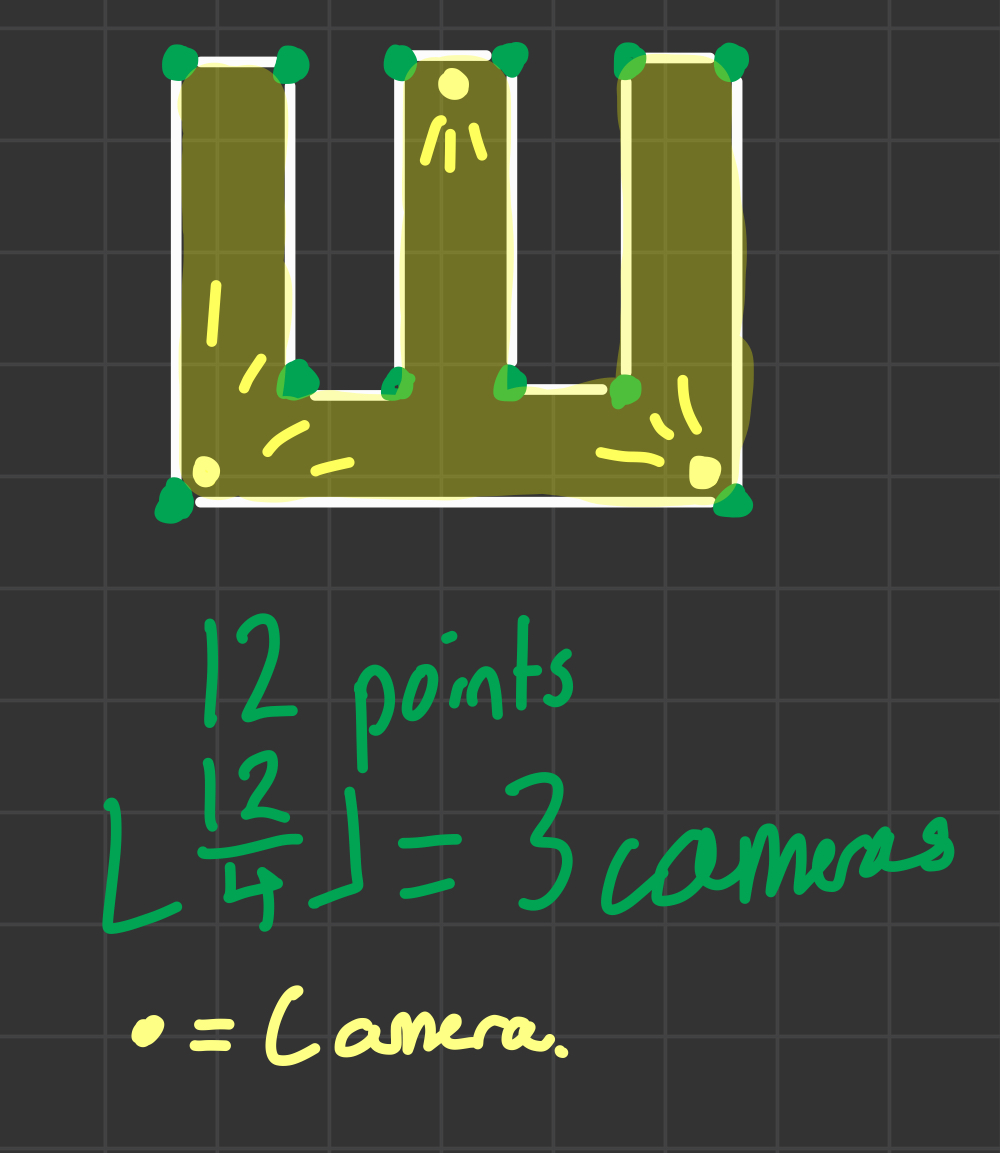
\includegraphics[scale =0.2]{3.2.jpeg}
    \end{center}
    \item[] If you were to add another "spike" to the polygon below it would add 4 more vertex and 1 more camera.
\end{itemize}
\end{document}